\section{Các Hệ Tọa độ trong Thị giác Máy tính}
\label{sec:coordinate_systems}

Để mô tả một cách chính xác quá trình một điểm trong thế giới ba chiều được chiếu lên mặt phẳng ảnh, việc định nghĩa rõ ràng các hệ tọa độ là điều bắt buộc. Một trong những nguồn gốc phổ biến của sai sót trong thị giác máy tính không nằm ở các công thức phức tạp, mà ở việc nhầm lẫn giữa các hệ tọa độ khác nhau.

Trong thực tế, không tồn tại một hệ tọa độ duy nhất. Thay vào đó, một điểm 3D sẽ được biểu diễn qua nhiều hệ tọa độ trung gian khác nhau, mỗi hệ phục vụ một mục đích riêng trong quá trình tạo ảnh. Việc hiểu rõ vai trò và mối quan hệ giữa các hệ này là chìa khóa để xây dựng mô hình camera một cách chính xác \cite{Hartley2003, Szeliski2010}.

Quan trọng hơn, các hệ tọa độ này không chỉ là công cụ biểu diễn, mà còn phản ánh các bước vật lý và toán học thực sự xảy ra trong quá trình tạo ảnh: từ vị trí của vật thể trong thế giới, đến cách camera "nhìn thấy" nó, rồi cách nó được chiếu lên mặt phẳng ảnh, và cuối cùng là cách nó được số hóa thành pixel.

\subsection{Tổng quan các Hệ Tọa độ}
\label{subsec:coordinate_overview}

Quá trình tạo ảnh có thể được xem như một chuỗi biến đổi tuần tự qua bốn hệ tọa độ chính:

\begin{enumerate}
	\item \textbf{Hệ tọa độ Thế giới (World Coordinate System)}
	\item \textbf{Hệ tọa độ Camera (Camera Coordinate System)}
	\item \textbf{Hệ tọa độ Ảnh (Image Coordinate System)}
	\item \textbf{Hệ tọa độ Pixel (Pixel Coordinate System)}
\end{enumerate}

\begin{center}
	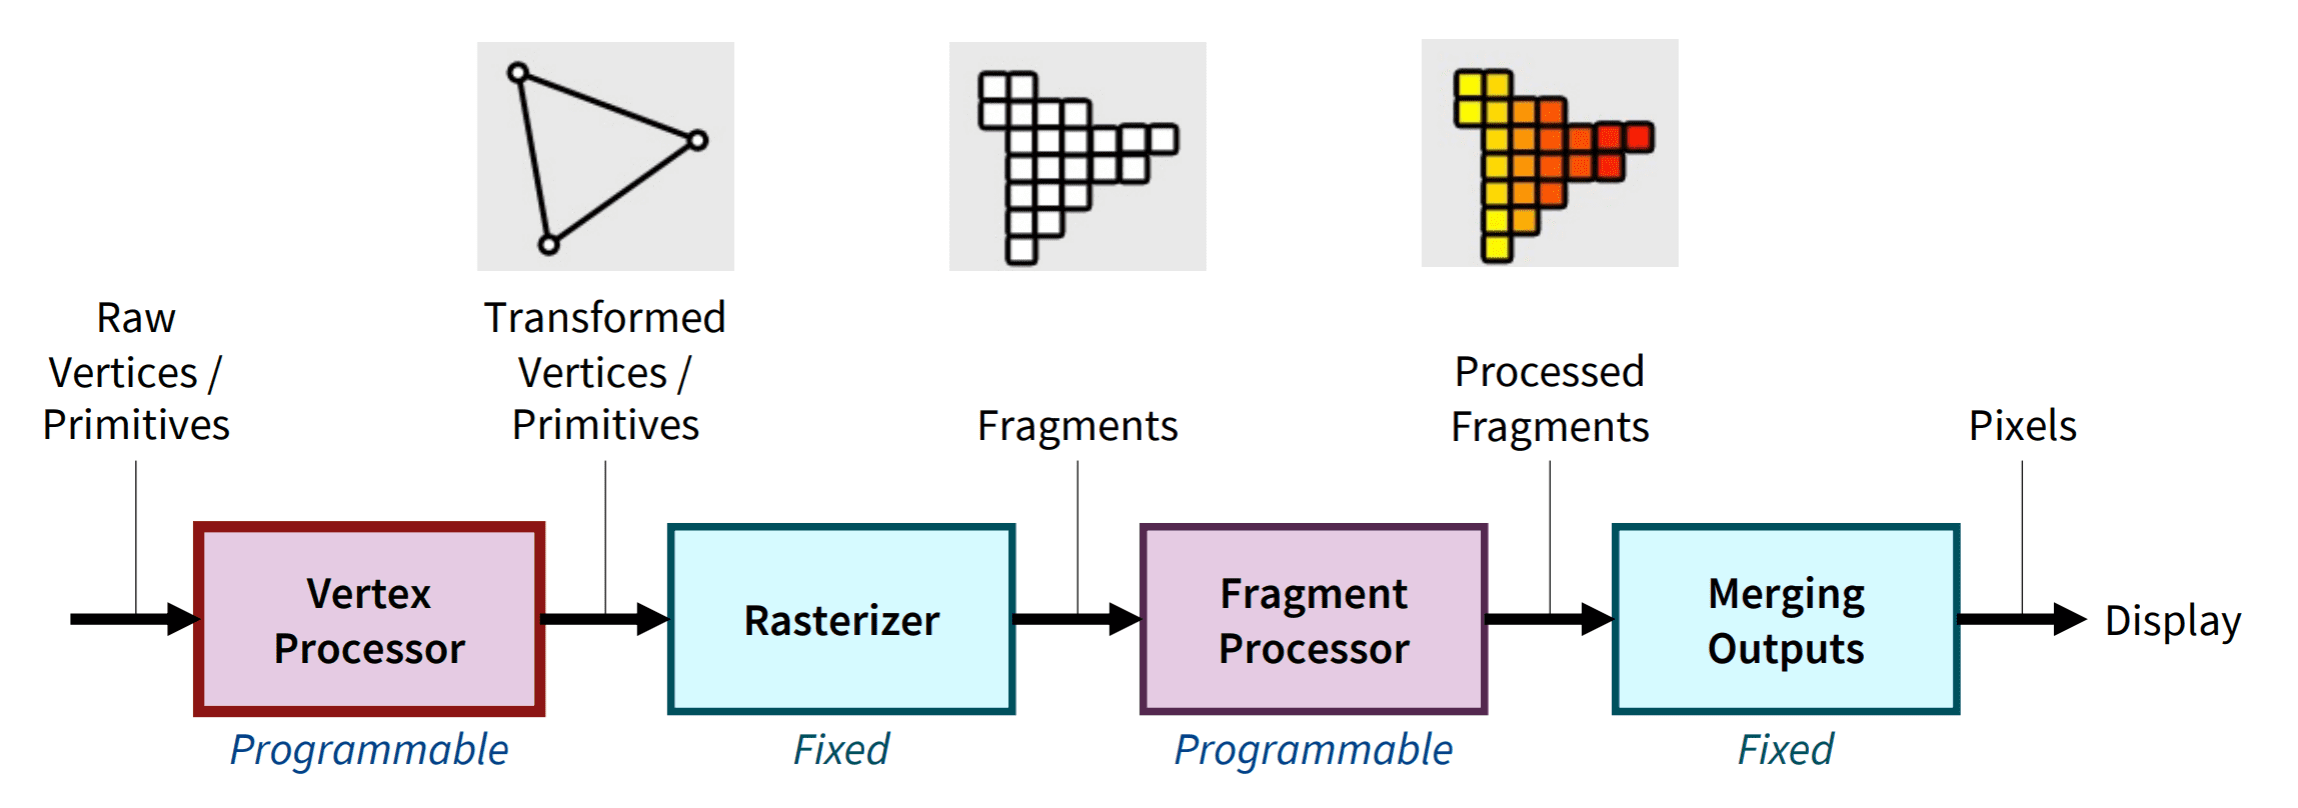
\includegraphics[width=0.85\textwidth]{images/coordinate_pipeline.png}
	\captionof{figure}{Chuỗi biến đổi từ thế giới 3D đến pixel 2D. Mỗi hệ tọa độ đóng vai trò như một bước trung gian trong quá trình tạo ảnh.}
	\label{fig:coordinate_pipeline}
\end{center}

Mỗi hệ tọa độ này đóng vai trò như một bước trung gian trong phép biến đổi tổng thể:

\[
\mathbf{P}_{world} \rightarrow \mathbf{P}_{camera} \rightarrow \mathbf{p}_{image} \rightarrow \mathbf{p}_{pixel}
\]

Điều quan trọng cần nhận thức là: mỗi mũi tên trong chuỗi trên không chỉ là một phép biến đổi toán học, mà còn tương ứng với một ý nghĩa vật lý cụ thể. Ví dụ, bước từ world sang camera thể hiện vị trí và hướng của camera, trong khi bước từ image sang pixel phản ánh cách cảm biến số hóa tín hiệu ánh sáng.

\subsection{Hệ tọa độ Thế giới}
\label{subsec:world_coordinate}

Hệ tọa độ thế giới là hệ tọa độ toàn cục, được sử dụng để mô tả cấu trúc của cảnh trong không gian 3D. Đây là hệ tọa độ mà trong đó các đối tượng thực tồn tại.

Một điểm trong không gian được biểu diễn dưới dạng:

\[
\mathbf{P}_w = (X_w, Y_w, Z_w, 1)^T
\]

Việc sử dụng tọa độ thuần nhất (thành phần $1$ ở cuối) cho phép chúng ta biểu diễn các phép biến đổi affine (quay, tịnh tiến) dưới dạng ma trận, giúp đơn giản hóa đáng kể việc tính toán.

\begin{mdframed}[style=infobox]
	\textbf{Trực giác: Hệ tọa độ "tuyệt đối"}
	
	Hệ tọa độ thế giới giống như một bản đồ toàn cục. Mọi vật thể đều có vị trí cố định trong hệ này, độc lập với vị trí của camera. Ví dụ, trong một hệ thống robot, đây có thể là hệ tọa độ gắn với môi trường hoặc bản đồ SLAM.
\end{mdframed}

Điểm quan trọng là hệ tọa độ thế giới là \textbf{tùy ý lựa chọn}. Không có một hệ chuẩn duy nhất, miễn là tất cả các đối tượng được biểu diễn nhất quán trong cùng một hệ.

Tuy nhiên, việc lựa chọn hệ tọa độ hợp lý có thể giúp đơn giản hóa bài toán. Ví dụ, trong nhiều trường hợp, người ta chọn hệ tọa độ sao cho một đối tượng quan trọng nằm tại gốc, hoặc các trục trùng với các hướng chính của môi trường.

\subsection{Hệ tọa độ Camera}
\label{subsec:camera_coordinate}

Hệ tọa độ camera được gắn trực tiếp với camera. Trong hệ này:

\begin{itemize}
	\item Gốc tọa độ nằm tại tâm camera $C$
	\item Trục $Z$ hướng ra phía trước (theo hướng nhìn)
	\item Trục $X$ và $Y$ song song với mặt phẳng ảnh
\end{itemize}

Một điểm trong hệ này được biểu diễn:

\[
\mathbf{P}_c = (X_c, Y_c, Z_c, 1)^T
\]

Mối quan hệ giữa hệ tọa độ thế giới và hệ tọa độ camera được mô tả bởi:

\[
\mathbf{P}_c = R \mathbf{P}_w + t
\]

hoặc trong dạng thuần nhất:

\[
\mathbf{P}_c = 
\begin{bmatrix}
	R & t \\
	0 & 1
\end{bmatrix}
\mathbf{P}_w
\]

trong đó:
\begin{itemize}
	\item $R$ là ma trận quay ($3 \times 3$)
	\item $t$ là vector tịnh tiến ($3 \times 1$)
\end{itemize}

\begin{center}
	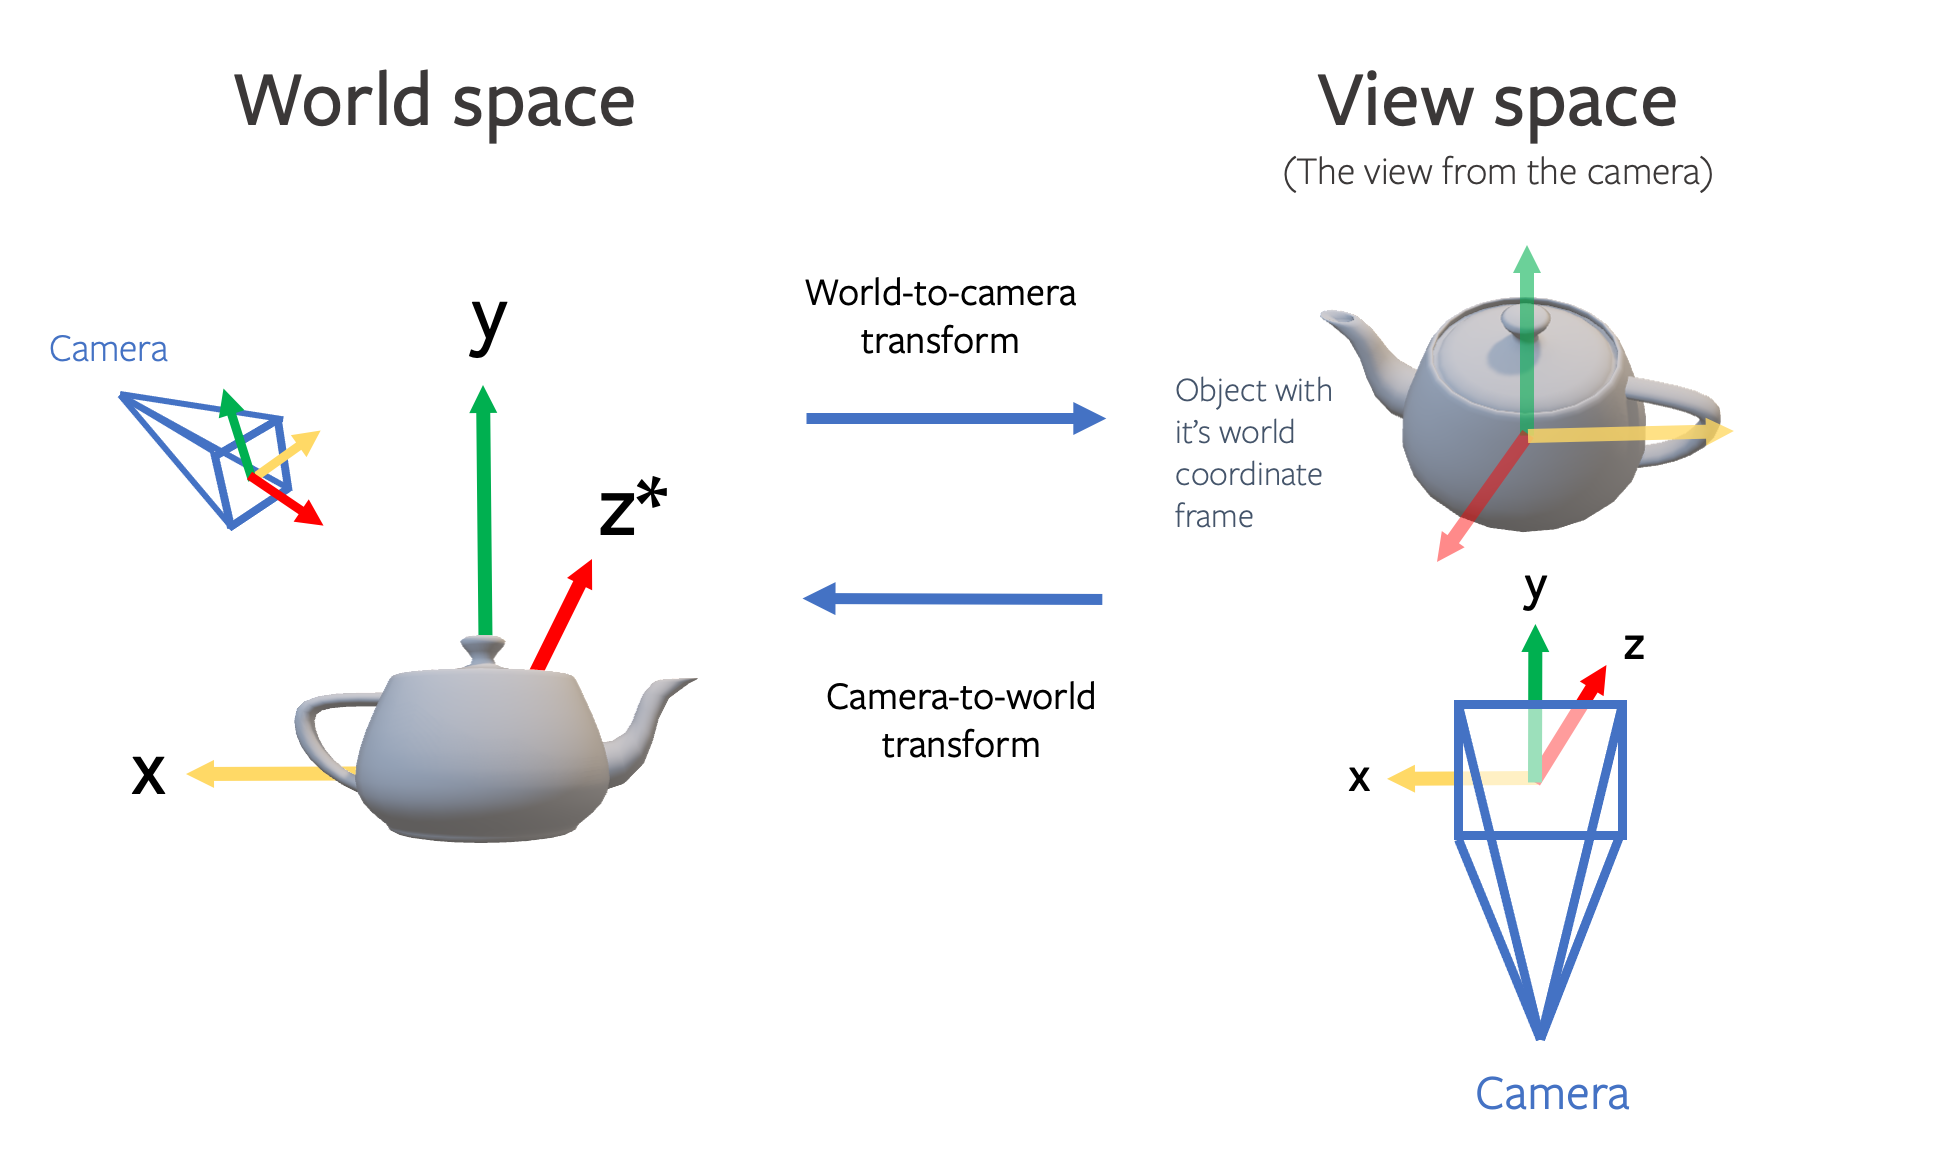
\includegraphics[width=0.75\textwidth]{images/world_to_camera.png}
	\captionof{figure}{Biến đổi từ hệ tọa độ thế giới sang hệ tọa độ camera. Camera được coi là cố định, và thế giới được biến đổi vào hệ của nó.}
	\label{fig:world_to_camera}
\end{center}

\begin{mdframed}[style=infobox]
	\textbf{Trực giác: "Di chuyển thế giới, không phải camera"}
	
	Mặc dù trực giác cho rằng camera di chuyển trong thế giới, về mặt toán học, chúng ta thường giữ camera cố định và "di chuyển" toàn bộ thế giới vào hệ tọa độ của camera thông qua $(R, t)$.
	
	Cách nhìn này giúp đơn giản hóa biểu diễn và là quy ước tiêu chuẩn trong thị giác máy tính \cite{Hartley2003}.
\end{mdframed}

Một điểm quan trọng cần lưu ý là $R$ và $t$ không chỉ là các tham số toán học, mà còn mang ý nghĩa vật lý rõ ràng: chúng mô tả tư thế (pose) của camera trong không gian. Việc ước lượng chính xác các tham số này là một bài toán trung tâm trong nhiều ứng dụng như SLAM và tái tạo 3D.

\subsection{Hệ tọa độ Ảnh}
\label{subsec:image_coordinate}

Sau khi được biểu diễn trong hệ tọa độ camera, điểm 3D được chiếu lên mặt phẳng ảnh thông qua phép chiếu phối cảnh:

\[
x = \frac{X_c}{Z_c}, \quad y = \frac{Y_c}{Z_c}
\]

Hệ tọa độ ảnh $(x, y)$:
\begin{itemize}
	\item Có gốc tại tâm ảnh (principal point)
	\item Được đo theo đơn vị vật lý (ví dụ: mm)
	\item Không phải là pixel
\end{itemize}

Đây là hệ tọa độ "liên tục", phản ánh trực tiếp hình học của phép chiếu.

\begin{center}
	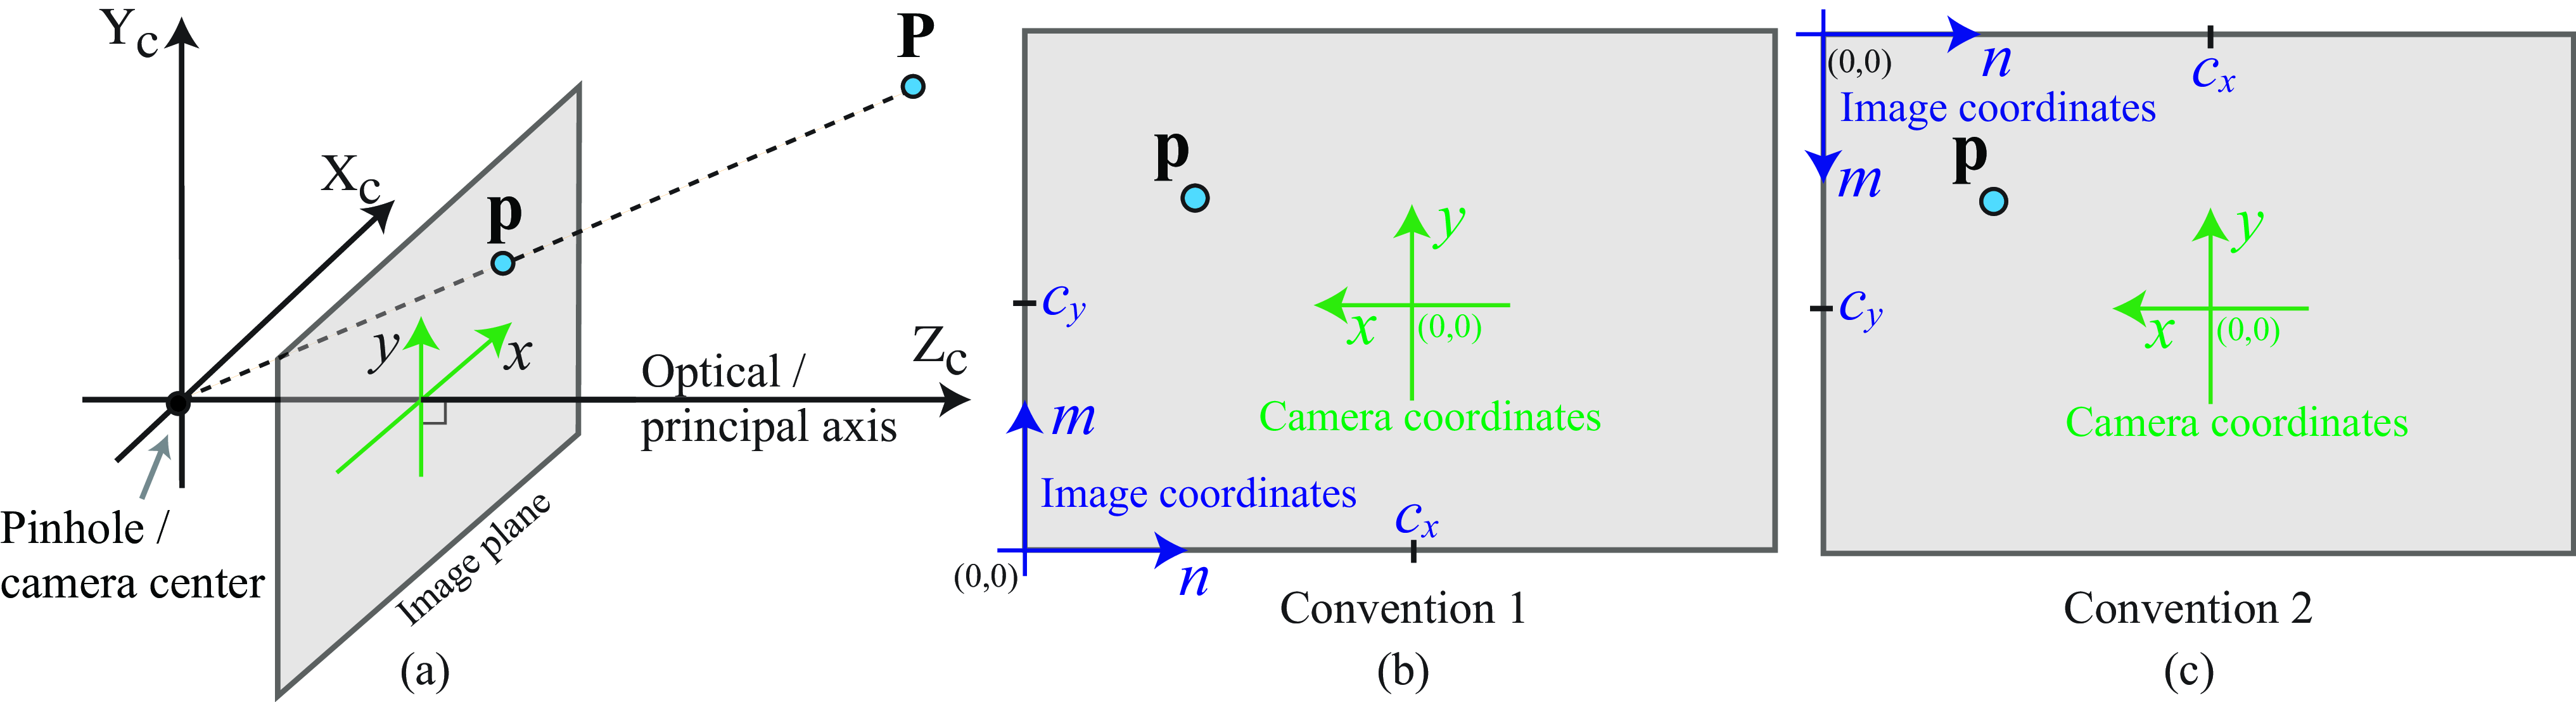
\includegraphics[width=0.75\textwidth]{images/image_plane_coordinates.png}
	\captionof{figure}{Hệ tọa độ ảnh trên mặt phẳng chiếu. Các tọa độ $(x, y)$ là liên tục và chưa bị rời rạc hóa thành pixel.}
	\label{fig:image_coordinates}
\end{center}

Điều quan trọng cần hiểu là hệ tọa độ này vẫn mang tính "lý tưởng". Nó chưa tính đến việc ảnh được lấy mẫu rời rạc bởi cảm biến. Do đó, đây là cầu nối giữa hình học liên tục và dữ liệu số.

\subsection{Hệ tọa độ Pixel}
\label{subsec:pixel_coordinate}

Cuối cùng, tọa độ ảnh được chuyển đổi sang hệ tọa độ pixel:

\[
u = f_x x + c_x, \quad v = f_y y + c_y
\]

Trong đó:
\begin{itemize}
	\item $(u, v)$ là tọa độ pixel
	\item $(f_x, f_y)$ là tiêu cự theo đơn vị pixel
	\item $(c_x, c_y)$ là tâm ảnh (principal point)
\end{itemize}

Khác với hệ tọa độ ảnh:
\begin{itemize}
	\item Gốc thường nằm ở góc trên bên trái
	\item Trục $v$ hướng xuống dưới
	\item Đơn vị là pixel (rời rạc)
\end{itemize}

\begin{center}
	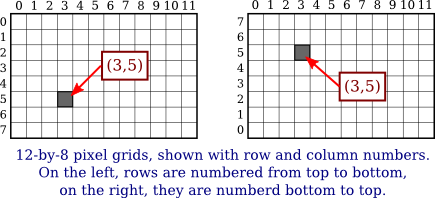
\includegraphics[width=0.75\textwidth]{images/pixel_coordinates.png}
	\captionof{figure}{Hệ tọa độ pixel với gốc ở góc trên bên trái. Trục $v$ hướng xuống dưới, khác với hệ tọa độ toán học truyền thống.}
	\label{fig:pixel_coordinates}
\end{center}

Sự chuyển đổi này thực chất là một phép biến đổi affine, chuyển từ hệ tọa độ vật lý sang hệ tọa độ số. Nó phản ánh đặc tính của cảm biến và cách dữ liệu được lưu trữ trong bộ nhớ.

\begin{mdframed}[style=infobox]
	\textbf{Cảnh báo: Một nguồn lỗi phổ biến}
	
	Việc nhầm lẫn giữa hệ tọa độ ảnh và hệ tọa độ pixel là một trong những lỗi phổ biến nhất. Đặc biệt, sự khác biệt về hướng trục $y$ (lên trên vs xuống dưới) có thể dẫn đến các lỗi khó phát hiện trong thực nghiệm.
\end{mdframed}

\subsection{Tổng hợp: Chuỗi Biến đổi Hoàn chỉnh}
\label{subsec:full_pipeline}

Kết hợp tất cả các bước, ta có chuỗi biến đổi hoàn chỉnh:

\[
\mathbf{p} = K [R|t] \mathbf{P}
\]

trong đó:
\begin{itemize}
	\item $[R|t]$ chuyển từ world $\rightarrow$ camera
	\item $K$ chuyển từ image $\rightarrow$ pixel
\end{itemize}

Một cách nhìn sâu hơn, phương trình này là sự kết hợp của hai loại biến đổi:
\begin{itemize}
	\item \textbf{Biến đổi ngoại tại (extrinsic)}: mô tả vị trí và hướng của camera
	\item \textbf{Biến đổi nội tại (intrinsic)}: mô tả cách camera tạo ảnh
\end{itemize}

Sự tách biệt này không chỉ có ý nghĩa về mặt toán học, mà còn rất quan trọng trong thực tế, đặc biệt trong các bài toán hiệu chỉnh camera (camera calibration).

\subsection{Kết luận}
\label{subsec:coordinate_conclusion}

Các hệ tọa độ không chỉ là một chi tiết kỹ thuật, mà là ngôn ngữ mà chúng ta sử dụng để mô tả hình học của quá trình tạo ảnh. Việc hiểu rõ từng hệ và cách chúng liên kết với nhau giúp tránh những sai lầm tinh vi và cung cấp nền tảng vững chắc cho các khái niệm nâng cao hơn như hiệu chỉnh camera và hình học đa ảnh.

Quan trọng hơn, việc thành thạo các hệ tọa độ cho phép chúng ta chuyển đổi linh hoạt giữa các góc nhìn khác nhau: từ thế giới vật lý sang biểu diễn toán học, và từ đó sang dữ liệu số mà máy tính có thể xử lý. Đây chính là cầu nối giữa thực tế và thuật toán trong Thị giác Máy tính.

\section*{Tài liệu tham khảo}
\begin{itemize}
	\item[1] Hartley, R., \& Zisserman, A. (2003). \textit{Multiple View Geometry in Computer Vision}. Cambridge University Press.
	\item[2] Szeliski, R. (2010). \textit{Computer Vision: Algorithms and Applications}. Springer.
\end{itemize}